\subsubsection{Configuración General}
Esta página web cuenta con una sección llamada \textit{Camino de Audio}, la cual cuenta con 4 botones que nos permiten seleccionar tanto la entrada, Radio o MP3, tanto la salida de audio, Auriculares o Altavoz.

También cuenta con una sección llamada \textit{Bajo Consumo} que cuenta con tan solo un botón que nos permitirá poner el microcontrolador en modo bajo consumo.

Por último, cuenta con una sección llamada \textit{Consumo}, que contiene un widget, el cual se ha obtenido de \textbf{REFENCIA A DE DONDE SE SACO ESTO} que nos permite visualizar de forma dinámica en consumo medido en el sistema. %REFERENCIA: WEB/ANIMACIONCONSUMO

\begin{figure}[h]
    \centering
    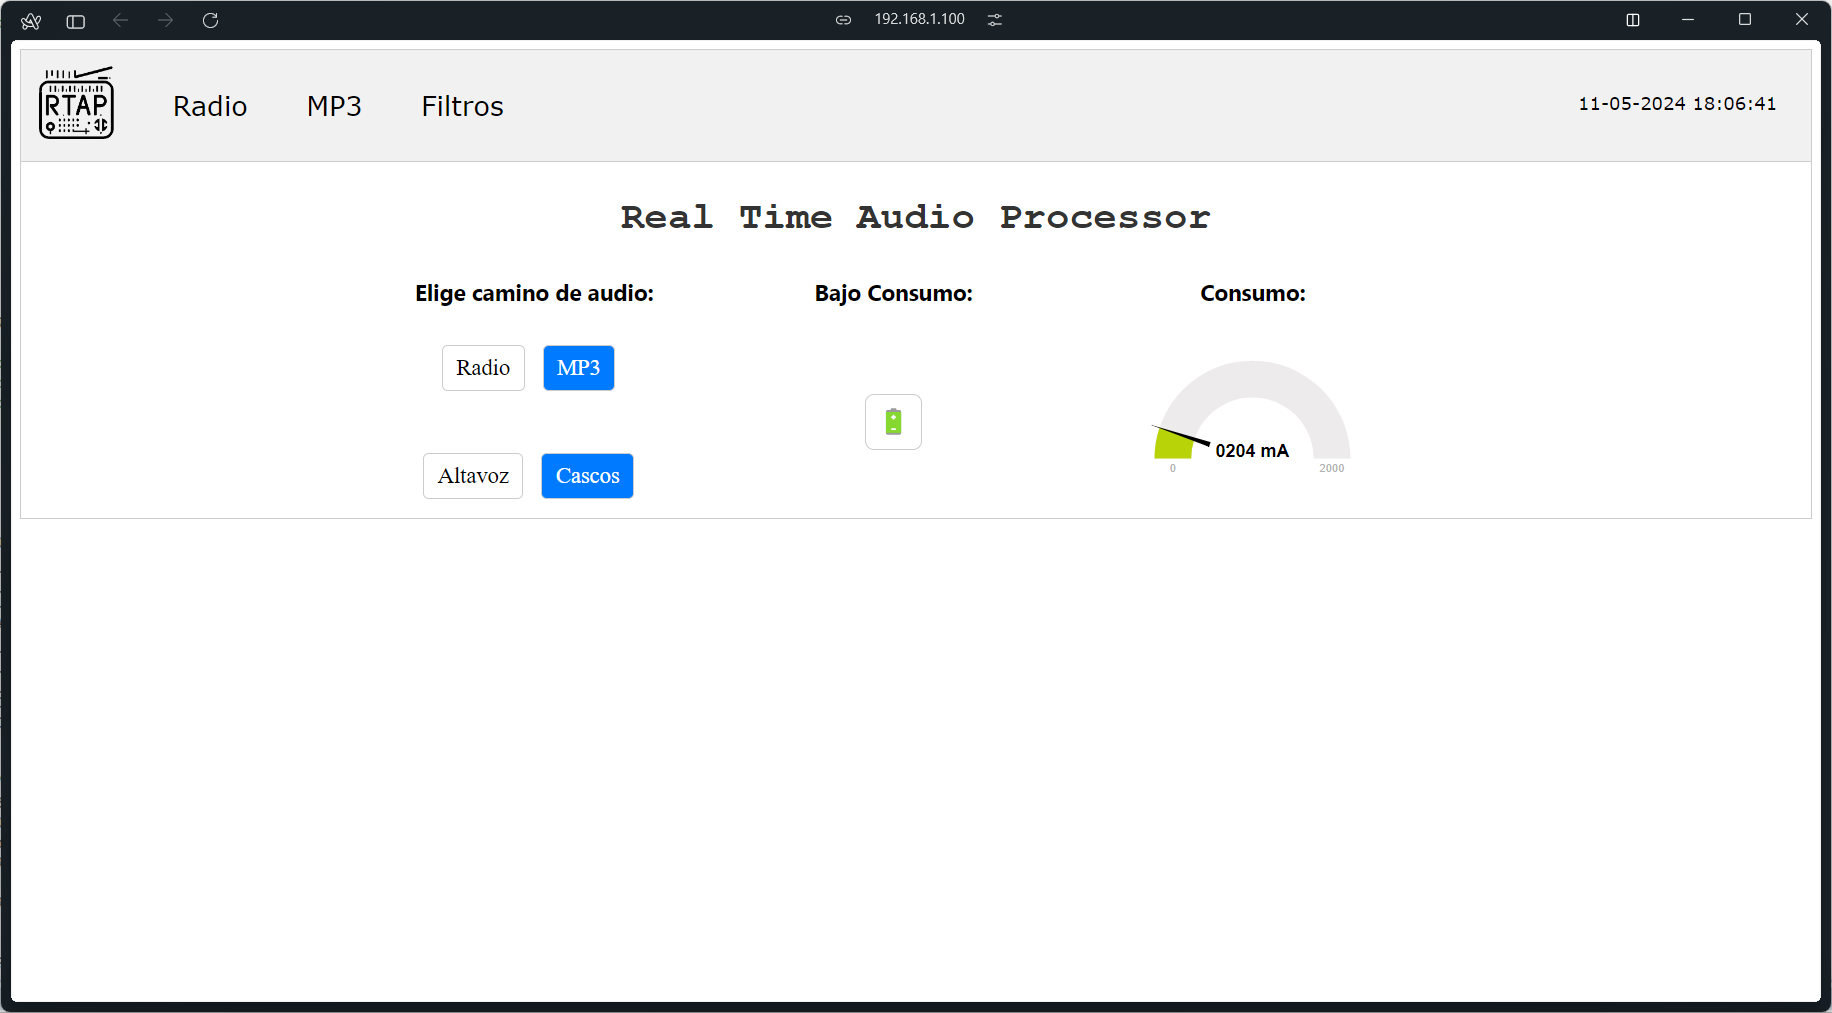
\includegraphics[width=0.8\textwidth]{images/3/3-1/3-1-1-1/Pagina_Principal.png}
    \caption{Página Principal}
    \label{fig:3-1-1-1-Principal}
\end{figure}